\documentclass[letterpaper, 11pt]{report}

\usepackage[utf8]{inputenc}
\usepackage[english, spanish]{babel}

\usepackage{fullpage}
\usepackage{graphicx}
\usepackage{amsmath}
\usepackage{enumitem}
\usepackage{chngcntr}
\usepackage{setspace}
\usepackage{xurl}
\usepackage{csquotes}
\usepackage{float}
\usepackage{verbatim}
\usepackage{tabularx}
\usepackage{amsmath}
\usepackage{caption}
\usepackage{bm}
\usepackage{wrapfig}
\usepackage{siunitx}
\usepackage{array}
\usepackage{enumitem}
\usepackage{longtable}



% \usepackage[margin=0.5in]{geometry}

\counterwithin{figure}{section}
\renewcommand{\thesection}{\arabic{section}}
\renewcommand{\thesubsection}{\thesection.\arabic{subsection}}
\renewcommand{\baselinestretch}{1.5}
\renewcommand{\thefigure}{\arabic{figure}}

\usepackage[style=apa, maxnames=6, minnames=3]{biblatex}
\DefineBibliographyStrings{english}{%chktex-file 1 chktex-file 6
      andothers = {\em et\addabbrvspace al\adddot}
}

\addbibresource{./Bibliography/bibliography.bib}


\setlength{\parskip}{\baselineskip}

\newcommand{\bolditalic}[1]{\textbf{\textit{#1}}}

\renewcommand{\comment}[1]{{\small $\ll$#1$\gg$}}

\renewcommand{\arraystretch}{1.3}
\setlength{\LTpre}{0pt}
\setlength{\LTpost}{0pt}

% chktex-file 8
% chktex-file 24
% chktex-file 44

\begin{document}

\begin{titlepage}
      \centering
      
\includegraphics[width=0.3\textwidth]{Images/logo_utb.png}\par\vspace{1cm}
      {\scshape\LARGE Universidad Tecnológica de Bolívar \par}
      \vspace{1cm}

      {\scshape\Large Formulación y Evaluación de Proyectos \par}
      \vspace{1cm}

      \slshape {\Large \bfseries{} Avance Proyecto \\}
      \vspace{2cm}

      \slshape {\itshape{} Valentina Daniela Del Rio Jimenez, T00081360 \\}
      \slshape {\itshape{} Mauro Alonso Gonzalez Figueroa, T00067622 \\}
      \slshape {\itshape{} Juan Jose Jimenez Guardo, T000 \\}
      \slshape {\itshape{} Jorge Alberto Rueda Salgado, T00068722 \\}
      \slshape {\itshape{} Joseph Gutiérrez de Piñeres, T00078923  \\}
      \slshape {\itshape{} Isaac Navarro, T00068237  \\}

      \vfill
      Revisado Por \\
      Leinys Melgarejo Causado\\
      {\large \today\par}
\end{titlepage}

\nocite{*}

\tableofcontents{}
\newpage

% !--------------------------------------------------------------------------------------|>
\section{Introducción}

El acceso a alimentos a precios justos dentro de las instituciones educativas
es un factor clave para el bienestar y el rendimiento académico de los
estudiantes. En muchas universidades, los altos costos de los insumos
alimenticios representan una carga económica significativa para la comunidad
estudiantil, limitando sus opciones de alimentación y afectando su calidad de
vida.

Este documento presenta un análisis detallado sobre la problemática del alto
costo de los insumos alimenticios en la universidad, identificando sus causas,
actores clave involucrados y posibles estrategias de solución. A través de un
enfoque estructurado, se evalúan diferentes alternativas para reducir los
costos de los alimentos dentro del campus, garantizando su accesibilidad sin
comprometer la calidad ni la sostenibilidad financiera de los proveedores.

% !--------------------------------------------------------------------------------------|>
\section{Descripción de la empresa}

La presente propuesta se desarrolla en el contexto de la universidad, que
funciona como el principal espacio de consumo de los insumos alimenticios
analizados en este estudio. La institución cuenta con un sistema de
concesionarios encargados de la venta de alimentos dentro del campus, los
cuales operan bajo contratos de concesión regulados por la administración
universitaria.

La universidad tiene como misión ofrecer una educación integral, promoviendo el
bienestar de su comunidad estudiantil a través de servicios complementarios
como el acceso a alimentación dentro del campus. Su visión es consolidarse como
una institución de referencia en la formación académica y en la generación de
condiciones óptimas para el desarrollo de sus estudiantes.

Actualmente, la estructura organizativa de la universidad está compuesta por
distintos departamentos administrativos, entre los cuales se encuentra el área
encargada de la regulación de concesionarios y servicios estudiantiles. Los
proveedores de alimentos dentro del campus forman parte de un modelo de negocio
basado en la venta directa a la comunidad estudiantil, con precios establecidos
según acuerdos comerciales y políticas internas.

El mercado objetivo de estos concesionarios está compuesto por estudiantes,
docentes y personal administrativo, quienes diariamente adquieren productos
dentro de las instalaciones. Sin embargo, la falta de regulación efectiva en
los precios ha generado una problemática que impacta directamente en la
economía de los estudiantes, afectando su acceso a una alimentación adecuada.

Este estudio busca analizar esta situación y proponer estrategias para mejorar
la accesibilidad de los alimentos en la universidad, sin afectar la
sostenibilidad de los proveedores y garantizando condiciones justas para toda
la comunidad universitaria.

% !--------------------------------------------------------------------------------------|>
\section{Análisis del Entorno}

\subsection{Situaciones Problemáticas Identificadas}

\begin{itemize}
      \item Falta de iluminación en la vía Transversal 14, Turbaco.
      \item Mala gestión de los recursos destinados a la salud.
      \item Deterioro de la vía intermunicipal Turbaco-Cartagena.
      \item Tarifa excesiva en los precios de los insumos alimenticios vendidos por la
            Universidad.
      \item Reacción tardía de los Servicios de Emergencia en Turbaco.
\end{itemize}

\subsection{Priorización del Problema}

\begin{longtable}{|p{.2\linewidth}|p{.2\linewidth}|p{.2\linewidth}|p{.2\linewidth}|p{.1\linewidth}|}
      \caption{Análisis de problemáticas en Turbaco}                                                                                                                                                                      \\
      \hline
      \textbf{Problemáticas}                                                       & \textbf{Positivo (+)}                                                     & \textbf{Negativo (-)} & \textbf{Interesante (?)} & Total \\
      \hline
      \endfirsthead

      \hline
      \textbf{Problemáticas}                                                       & \textbf{Positivo (+)}                                                     & \textbf{Negativo (-)} & \textbf{Interesante (?)} & Total \\
      \hline
      \endhead

      \hline
      \endfoot

      \hline
      \endlastfoot

      Falta de iluminación en la vía Transversal 14, Turbaco                       & Mejora la seguridad
      reduciendo delitos nocturnos. Disminuye la tasa de accidentes de tránsito.
      Aumenta la calidad de vida de los habitantes.                                & Costos elevados de
      infraestructura y mantenimiento. Requiere permisos y aprobación de entidades
      gubernamentales. Posible vandalismo de luminarias recién instaladas.         & La
      iluminación puede incentivar el comercio nocturno. Puede influir en la
      plusvalía de las viviendas cercanas.                                         & $3 - 3 + 2 = 2$                                                                                                                      \\ \hline

      Mala gestión de los recursos destinados a la salud                           & Asegura mejor atención
      médica para la población. Optimiza el uso del presupuesto público. Reduce
      corrupción y mala administración en salud.                                   & Problema complejo que requiere
      reformas estructurales. Dificultades para obtener información transparente.
      Resistencia de actores con intereses en la mala gestión.                     & Puede generar
      presión social y movilización ciudadana. Comparaciones con otros municipios
      pueden ayudar a evidenciar el problema.                                      & $3 - 3 + 2 = 2$                                                                                                                      \\ \hline

      Deterioro de la vía intermunicipal Turbaco-Cartagena                         & Mejora la movilidad y
      reduce tiempos de desplazamiento. Disminuye costos en mantenimiento de
      vehículos. Beneficia la economía local y el turismo.                         & Costos elevados de
      reparación y mantenimiento. Requiere planificación de cierres viales, afectando
      la movilidad. Posibles demoras en ejecución de obras por burocracia o
      corrupción.                                                                  & Puede atraer inversión privada para su financiamiento. Aumenta el
      atractivo de Turbaco como zona residencial.                                  & $3 - 3 + 2 = 2$                                                                                                                      \\ \hline

      Tarifa excesiva en los precios de los insumos alimenticios vendidos por la
      Universidad                                                                  & Alivia la carga económica de los estudiantes. Puede fomentar
      hábitos alimenticios más saludables. Aumenta la satisfacción estudiantil y el
      rendimiento académico.                                                       & Resistencia de concesionarios y proveedores a reducir
      precios. Problema influenciado por la inflación y costos de importación.
      Difícil intervención directa de la universidad sin afectar contratos vigentes.
                                                                                   & Las universidades con precios justos tienen mejor percepción estudiantil.
      Puede promover la competencia con opciones externas más económicas. Posible
      implementación de subsidios o descuentos para estudiantes de bajos recursos. &
      $3 - 3 + 3 = 3$                                                                                                                                                                                                     \\ \hline

      Reacción tardía de los Servicios de Emergencia en Turbaco                    & Reduce muertes y
      complicaciones médicas. Genera confianza en el sistema de salud. Mejora la
      eficiencia operativa de ambulancias y hospitales.                            & Necesidad de más
      ambulancias y personal capacitado. Problemas logísticos como vías
      congestionadas o en mal estado. Posible falta de presupuesto para mejorar los
      tiempos de respuesta.                                                        & La tecnología (apps de emergencia, GPS) puede optimizar
      la respuesta. Colaboración con voluntarios o bomberos podría mejorar la
      cobertura.                                                                   & $3 - 3 + 2 = 2$                                                                                                                      \\
\end{longtable}

Se ha determinado que la problemática prioritaria es el alto costo de los
insumos alimenticios dentro de la universidad. Este problema impacta
directamente la economía de los estudiantes y su acceso a una alimentación
adecuada, lo que puede repercutir en su bienestar y rendimiento académico.

\subsection{Identificación de Actores Clave}

\begin{itemize}
      \item  Administración Universitaria: Responsable de la concesión y regulación de los
            servicios de cafetería y venta de alimentos.
      \item  Proveedores y concesionarios de alimentos: Encargados de la compra,
            distribución y comercialización de los insumos alimenticios dentro de la
            universidad.
      \item  Estudiantes y comunidad universitaria: Afectados directos por los altos costos
            de los alimentos.
      \item  Organismos de control y defensa del consumidor: Entidades que pueden intervenir
            en la regulación de precios y calidad de los productos.
      \item  Gobierno y sector privado: Posibles aliados en la implementación de subsidios o
\end{itemize}

\subsection{Análisis del Problema y Objetivos}

\subsubsection{Árbol del Problema}

\begin{figure}[H]
      \begin{center}
            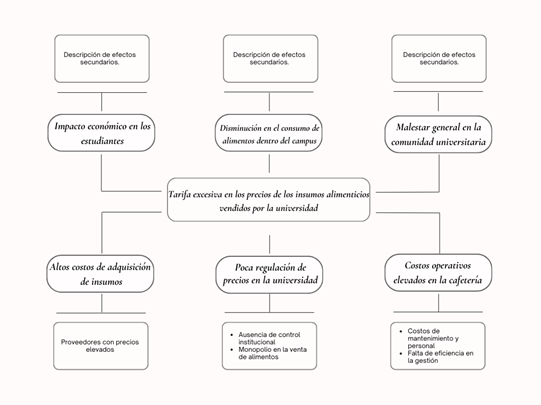
\includegraphics[width=\linewidth]{./Images/arbol_problema.png}
            \caption{}
      \end{center}
\end{figure}

\subsubsection{Árbol de Objetivos}

\begin{figure}[H]
      \begin{center}
            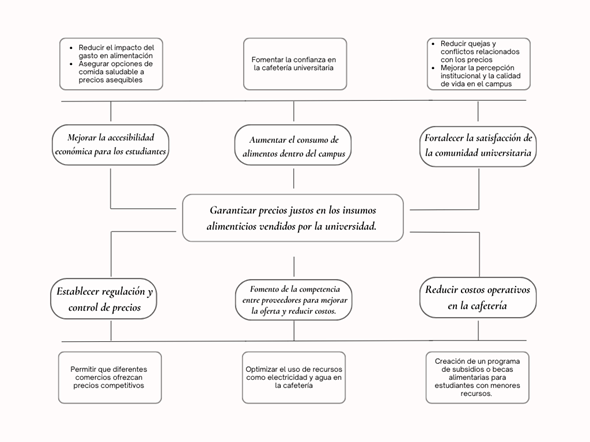
\includegraphics[width=\linewidth]{./Images/arbol_objetivo.png}
            \caption{}
      \end{center}
\end{figure}

% !--------------------------------------------------------------------------------------|>
\section{Evaluación de Alternativas de Solución}

\subsection{Regulación de precios}

\begin{itemize}
      \item Implementación gradual: Establecer un periodo de ajuste para que los
            proveedores se adapten al nuevo régimen de precios.

      \item Monitoreo continuo: Implementar un sistema automatizado para verificar los
            precios regularmente y ajustar según sea necesario.

      \item Incentivos fiscales: Ofrecer incentivos fiscales a los proveedores que cumplan
            con los precios establecidos.
\end{itemize}

\subsection{Educación y transparencia}

Crear campañas educativas para estudiantes y proveedores sobre los beneficios
de precios regulados para la comunidad universitaria.

\subsection{Flexibilidad en condiciones}

Permitir cierta flexibilidad en los precios para productos estacionales o
sujetos a fluctuaciones de mercado.

\subsection{Fomento de la competencia}

\begin{itemize}
      \item \textbf{Talleres y capacitaciones}: Ofrecer capacitaciones y talleres para nuevos
            concesionarios interesados en participar en licitaciones.
      \item \textbf{Acceso a información}: Publicar detalles sobre las licitaciones de manera
            accesible y transparente.
      \item \textbf{Evaluación objetiva}: Establecer criterios claros y objetivos para evaluar
            propuestas de nuevos concesionarios.
      \item \textbf{Periodicidad en licitaciones}: Realizar licitaciones periódicas para mantener un
            mercado dinámico.
      \item \textbf{Apoyo logístico}: Facilitar el acceso a infraestructura y recursos necesarios
            para nuevos entrantes.

\end{itemize}

\subsection{Creación de un comedor subsidiado}

\begin{itemize}
      \item \textbf{Estudios de mercado}: Realizar estudios de mercado para determinar la demanda y
            preferencias alimentarias de los estudiantes.
      \item \textbf{Alianzas estratégicas}: Colaborar con entidades gubernamentales y privadas para
            asegurar financiamiento sostenible.
      \item \textbf{Programas de becas alimenticias}: Establecer programas de becas para estudiantes
            en necesidad extrema.
      \item \textbf{Monitoreo de calidad}: Implementar controles estrictos de calidad en los
            alimentos ofrecidos.
      \item \textbf{Sostenibilidad financiera}: Desarrollar modelos financieros que garanticen la
            viabilidad a largo plazo del comedor subsidiado.

\end{itemize}

\subsection{Convenios con proveedores locales}

\begin{itemize}
      \item \textbf{Reducción de intermediarios}: Facilitar acuerdos directos entre la universidad y los proveedores locales.
      \item \textbf{Transporte eficiente}: Optimizar rutas de transporte para minimizar costos logísticos.
      \item \textbf{Certificación de productos}: Establecer estándares de calidad y certificación para los productos locales.
      \item \textbf{Promoción de productos locales}: Realizar campañas para promover la compra de productos locales entre la comunidad universitaria.
      \item \textbf{Flexibilidad en contratos}: Ofrecer contratos flexibles que se ajusten a las necesidades cambiantes de los proveedores locales.
\end{itemize}

\subsection{Control y auditoría}

\begin{itemize}
      \item  \textbf{Auditorías independientes}: Contratar firmas de auditoría externas para realizar
            evaluaciones periódicas.
      \item  \textbf{Feedback de usuarios}: Implementar sistemas de retroalimentación para
            estudiantes sobre la calidad y precios de los alimentos.
      \item  \textbf{Transparencia total}: Publicar resultados de auditorías de manera accesible para
            la comunidad universitaria.
      \item  \textbf{Sanciones por incumplimiento}: Establecer medidas correctivas y sanciones claras
            para proveedores que no cumplan con los estándares establecidos.
      \item  \textbf{Capacitación en cumplimiento}: Ofrecer capacitaciones regulares a los
            proveedores sobre las políticas de control y auditoría.
\end{itemize}

% !--------------------------------------------------------------------------------------|>
\section{Plan de Implementación}

Para asegurar el éxito de la estrategia elegida, se plantea el siguiente plan
de acción:

\begin{enumerate}
      \item \textbf{Diagnóstico inicial} (0$-$3 meses):
            \begin{itemize}
                  \item Realización de un estudio de costos y precios actuales en las cafeterías del
                        campus.
                  \item Identificación de proveedores y sus márgenes de ganancia.
                  \item Encuesta a estudiantes sobre su gasto en alimentación y nivel de satisfacción.
            \end{itemize}

      \item \textbf{Definición de políticas y alianzas} (4$-$6 meses):
            \begin{itemize}
                  \item Elaboración de una propuesta de regulación de precios y concesionarios.
                  \item Búsqueda de socios estratégicos para la implementación del comedor subsidiado.
                  \item Firma de acuerdos con proveedores locales para reducir costos.
            \end{itemize}

      \item \textbf{Ejecución de estrategias} (7$-$12 meses):
            \begin{itemize}
                  \item Aplicación de la regulación de precios en la universidad.
                  \item Inicio de operaciones del comedor subsidiado con tarifas diferenciadas.
                  \item Evaluación del impacto en el bienestar de los estudiantes.

            \end{itemize}

      \item \textbf{Monitoreo y ajustes} (12+ meses):

            \begin{itemize}
                  \item Revisión periódica de la efectividad de las medidas implementadas.
                  \item Ajuste de estrategias en función de los resultados obtenidos.
            \end{itemize}
\end{enumerate}

\subsection{Matriz Marco Lógico}

\begin{longtable}{|p{.2\linewidth}|p{.2\linewidth}|p{.3\linewidth}|p{.2\linewidth}|}
      \caption{Matrix Marco Logico}                                                                                                                                                                                   \\
      \hline
      \textbf{Elemento}                                                           & \textbf{Indicadores}                                                      & \textbf{Fuentes de Verificación} & \textbf{Supuestos} \\
      \hline
      \endfirsthead

      \hline
      \textbf{Elemento}                                                           & \textbf{Indicadores}                                                      & \textbf{Fuentes de Verificación} & \textbf{Supuestos} \\
      \hline
      \endhead

      \hline
      \endfoot

      \hline
      \endlastfoot

      Fin                                                                         & Mejora del bienestar estudiantil mediante el acceso a alimentos a precios
      justos.                                                                     & Encuestas de satisfacción estudiantil, informes académicos.               & Apoyo
      institucional y gubernamental.                                                                                                                                                                                  \\\hline

      Propósito                                                                   & Reducción del costo de los insumos alimenticios dentro del campus
      universitario.                                                              & Comparación de precios antes y después de la implementación de
      Componentesestrategias.                                                     & Disposición de proveedores y concesionarios a
      negociar precios.                                                                                                                                                                                               \\\hline

      Componentes                                                                 & Regulación de precios. Fomento de la competencia entre
      concesionarios. Creación de un comedor subsidiado. Establecimiento de convenios
      con proveedores locales. Implementación de auditorías y control de precios. &
      Acuerdos firmados con proveedores. Implementación de nuevas políticas de
      concesión. Creación de un sistema de control y auditoría.                   &                                                                                                                                   \\\hline

      Actividades                                                                 & Diagnóstico inicial sobre costos y precios. Búsqueda de aliados
      estratégicos. Diseño e implementación de estrategias de reducción de costos.
      Evaluación y monitoreo de los resultados.                                   & Informes de diagnóstico. Contratos
      y acuerdos. Reportes de seguimiento.                                        & Cooperación entre la universidad y los
      concesionarios.                                                                                                                                                                                                 \\\hline

\end{longtable}

\newpage
\subsection{Matriz De Plan de Estudio}

\begin{longtable}{|p{.2\linewidth}|p{.2\linewidth}|p{.3\linewidth}|p{.2\linewidth}|}
      \caption{Matriz De Plan de Estudio}                                                                                                                                                                                  \\
      \hline
      \textbf{Actividad}                           & \textbf{Descripción}                                                        & \textbf{Encargados}                      & \textbf{Tiempo \hfil{} \break{}Determinado}  \\
      \hline
      \endfirsthead

      \hline
      \textbf{Actividad}                           & \textbf{Descripción}                                                        & \textbf{Encargados}                      & \textbf{Tiempo \hfil{} \break{} Determinado} \\
      \hline
      \endhead

      \hline
      \endfoot

      \hline
      \endlastfoot

      1. Investigación de la situación alimentaria & Recolección de datos acerca de la
      población estudiantil y sus necesidades      & Grupo de trabajo/grupo de proyecto                                          &
      Una semana y media                                                                                                                                                                                                   \\\hline

      2. Análisis de Oferta y Demanda              & Identificar los factores de la oferta alimentaria y cual es la demanda real & Encargados de Investigación              & Una semana                                   \\\hline

      3. Identificar actores clave                 & Reconocimiento de instituciones, proveedores y posibles aliados             & Lider de grupo/líder del proyecto        & Cinco días                                   \\\hline

      4. Diseño de propuesta alimentaria           & Definición de la solución (comedor, convenios, subsidios)                   & Equipo de diseño/grupo de diseño         & Una semana                                   \\\hline

      5. Estudio Financiero Básico                 & Calcular costos, analizar fuentes de financiación y capital inicial         & Responsable financiero/Lider de proyecto & Dos semanas                                  \\hline

      6. Desarrollo del plan operativo             & Planeación de logística, recursos, tiempos. Ubicación y gestión             & Todo el equipo                           & Una semana                                   \\\hline

      7. Evaluación y ajustes                      & Retroalimentación sobre el proyecto y mejoras necesarias                    & Docente y Equipo                         & 3 días                                       \\\hline

      8. Presentación final del proyecto           & Elaboración final del documento y presentación de resultados                & Todo el equipo                           & 3 días                                       \\\hline

\end{longtable}

\section{Datos Demográficos}

Para el desarrollo del proyecto se ha elegido ubicación geográfica la ciudad
Cartagena Bolívar específicamente en la Universidad Tecnológica de Bolívar, una
institución de educación superior que acoge a estudiantes de diversos estratos
socioeconómicos, provenientes principalmente de la región Caribe.

\begin{enumerate}
      \item Ciudad, Distrito: Cartagena de Indias, Bolívar.
      \item Barrio: Ternera, Campus Lemaitre
      \item Localidad: Localidad 3 - Industrial y de la Bahía.
      \item Unidad Comunera: Unidad Comunera 13.
      \item Código DANE:\@{} 13001
      \item Zona: Urbana
      \item Forma Área: Campus universitario cerrado.
      \item Forma de Longitud: 10°24´59´´N
      \item Coordenadas: 10.4165°N,75.5336°W
\end{enumerate}

\subsection{Información sobre el sector estudiado}

El presente análisis se enfoca en el sector de servicios alimentarios dentro
del entorno universitario, un ámbito caracterizado por una demanda específica y
concentrada. La comunidad estudiantil requiere, primordialmente, opciones
alimenticias de rápida preparación que se ajusten a presupuestos limitados y, a
su vez, contribuyan a una dieta equilibrada y saludable. Este enfoque
particular del sector subraya la importancia de la accesibilidad económica y
nutricional como factores clave para satisfacer las necesidades de los
usuarios.

No obstante, se ha identificado una problemática significativa en este sector:
la existencia de barreras que impiden o dificultan el acceso universal a una
alimentación tanto económica como nutricionalmente adecuada para la comunidad
universitaria. Esta situación genera un entorno desfavorable que trasciende la
mera satisfacción de una necesidad básica, impactando directamente en aspectos
fundamentales de la vida universitaria. La dificultad para acceder a opciones
alimentarias saludables y asequibles puede deteriorar la calidad de vida de los
estudiantes, influir negativamente en su rendimiento académico y contribuir a
aumentar las desigualdades dentro del campus. Por lo tanto, este estudio se
enmarca en la comprensión de los servicios de consumo esenciales dentro de las
instituciones de educación superior, buscando analizar y comprender las
dinámicas de un sector crucial para el bienestar y el desarrollo integral de la
población universitaria.

\subsection{Demanda}

La comunidad universitaria presenta una alta demanda de servicios de
alimentación accesibles, saludables y eficientes. Esta necesidad responde a
condiciones como la carga académica, los horarios extensos y los recursos
económicos limitados, especialmente en los estudiantes de estratos bajos.

La demanda actual de servicios de alimentación por parte de la comunidad
universitaria no está siendo satisfecha adecuadamente, lo que se refleja en el
limitado uso de los servicios disponibles en el campus. Para responder a esta
necesidad, la propuesta plantea soluciones como subsidios, convenios con
entidades externas o la creación de un comedor universitario.

\subsection{Oferta}

La oferta actual dentro del campus universitario está compuesta por un conjunto
de concesionarios privados que operan bajo contratos de concesión con la
administración de la Universidad Tecnológica de Bolívar. Estos proveedores
ofrecen servicios de alimentación básica, sin embargo, presentan limitaciones
en cuanto a variedad de productos, precios competitivos y accesibilidad
económica para todos los estudiantes.

La oferta alimentaria actual en el campus universitario carece de opciones
saludables, menús para dietas específicas y precios asequibles. La falta de
regulación y competencia limita la mejora del servicio, y los estudiantes
tienen poca influencia. El proyecto busca mejorar y diversificar esta oferta
mediante un comedor subsidiado, acuerdos locales, incentivos por calidad y
precio, y programas de alimentación saludable asequible.

\subsection{Tendencia De Mercado}

En el contexto universitario, se observa una tendencia creciente hacia la
implementación de políticas de bienestar estudiantil enfocadas en garantizar el
acceso a servicios básicos como la alimentación, la salud mental y el
transporte. Esta tendencia responde a cambios socioeconómicos que afectan
directamente la capacidad de los estudiantes para mantenerse en el sistema
educativo, especialmente en sectores vulnerables.

Los estudiantes, especialmente de estratos bajos y con largas jornadas
académicas, demandan soluciones que les permitan permanecer en la universidad
sin tener que abandonar sus estudios por razones económicas. Por eso, las
instituciones están promoviendo estrategias alimentarias subsidiadas o
autogestionadas (comedores, vales alimentarios, convenios con restaurantes),
con un enfoque en la seguridad alimentaria y nutricional.

Además, factores como la inflación, el desempleo juvenil y los desafíos de
movilidad urbana también han influido en que los campus universitarios se
conviertan en espacios que ofrecen soluciones integrales al bienestar de los
estudiantes.

\subsection{Estrategias de Mercado}

La propuesta de valor del proyecto se basa en mejorar el acceso alimentario, a
través de alternativas más asequibles, saludables y óptimas para los
estudiantes universitarios. Dicha propuesta se alinea con una estrategia de
posicionamiento institucional, que refuerza el compromiso de la Universidad
Tecnológica De Bolívar con el bienestar de sus estudiantes.

Ahora bien, para lograr este objetivo, se implementa una estrategia de mercado,
la cual esta compuesta por los siguientes puntos clave:

\begin{enumerate}
      \item Diferenciación del servicio: \begin{itemize}
                  \item Ofrecer un comedor universitario con menús saludables y variados a precios
                        accesibles para todos los estudiantes.
                  \item Establecer colaboraciones con emprendimientos locales que ofrezcan opciones
                        alimenticias especializadas a precios preferenciales para la comunidad
                        universitaria
            \end{itemize}

      \item Segmentación y personalización: \begin{itemize}
                  \item Identificar las necesidades alimentarias y capacidad económica de los
                        estudiantes a través de encuestas y datos institucionales.
                  \item Aplicar precios diferenciadores y posibles subsidios para los estudiantes en
                        situación de vulnerabilidad.
            \end{itemize}

      \item Alianzas estratégicas: \begin{itemize}
                  \item Establecer convenios con proveedores locales para reducir costos de
                        intermediación.
                  \item Involucrar organizaciones no gubernamentales, instituciones públicas y
                        entidades privadas en la financiación o provisión de insumos.

            \end{itemize}

      \item Promoción institucional: \begin{itemize}
                  \item Realizar campañas de concientización dentro del campus sobre la importancia de
                        una alimentación saludable.
                  \item Utilizar canales institucionales (redes sociales, página web, correo
                        electrónico y eventos académicos) para informar sobre el nuevo servicio y sus
                        beneficios.

            \end{itemize}
\end{enumerate}

Con esta estrategia integral, se busca hacer posicionamiento del servicio
alimentario como una propuesta de alto valor, accesible y alineada con los
objetivos de desarrollo social y educativo de la universidad.

\subsection{Segmentación}

En este contexto, dicha segmentación nos permite dirigir de manera más
eficiente los esfuerzos hacia quienes más lo necesitan, priorizando a los
estudiantes en condición de vulnerabilidad económica y con mayor permanencia
dentro del campus universitario.

\subsection{Partes de la segmentación}

\begin{enumerate}
      \item Demográfica: Estudiantes universitarios entre 17 y 30 años, de estratos 1, 2 y
            3.
      \item Conducta: Jóvenes que buscan alimentación económica, saludable y nutritiva.
      \item Geográfica: Comunidad universitaria ubicada en el campus de la Universidad
            Tecnológica de Bolívar.

      \item Mercado meta: \begin{itemize}
                  \item  Estudiantes con recursos económicos limitados que permanecen largas jornadas en
                        la universidad.
                  \item  Personal administrativo y docente que consume alimentos en el campus

            \end{itemize}

      \item Posicionamiento: \textit{``Una alternativa alimentaria solidaria, saludable y
                  accesible para toda la comunidad universitaria''}
\end{enumerate}

\section{Mix de marketing (4P)}

\subsection{Producto}

Servicio de alimentación saludable y asequible (comedor universitario,
convenios con concesionarios o subsidios).

\subsection{Precio}

\begin{itemize}
      \item Tarifas subsidiadas o reguladas.
      \item Opciones variables para todos los estratos socioeconómicos.

\end{itemize}

\subsection{Plaza}

\begin{itemize}
      \item Campus universitario, con puntos de distribución estratégicos.
      \item Posibles alianzas con emprendimientos dirigidos a la universidad.
\end{itemize}

\subsection{Promoción}

\begin{itemize}
      \item Campañas internas de sensibilización.
      \item Difusión por redes institucionales, eventos universitarios y carteleras.
      \item Participación de grupos estudiantiles y bienestar universitario.
\end{itemize}

\subsection{Matrix FODA}

\begin{figure}[H]
      \begin{center}
            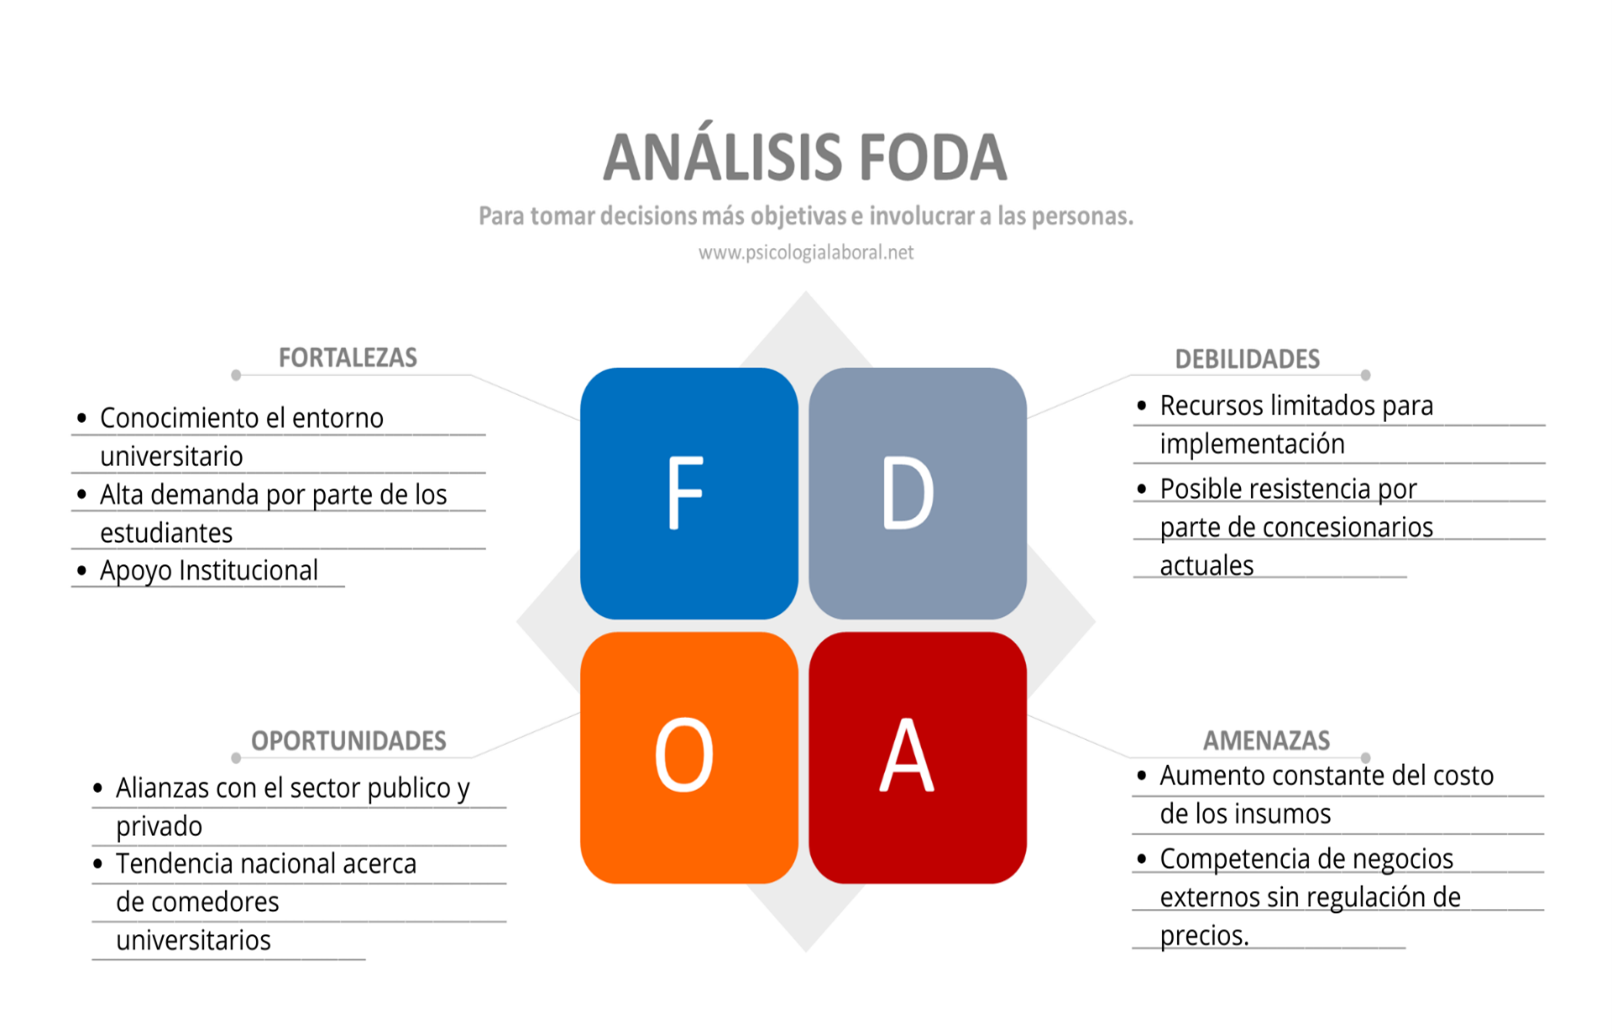
\includegraphics[width=\linewidth]{./Images/matrix_foda.png}
            \caption{}
      \end{center}
\end{figure}

En este proyecto La matriz FODA, se utiliza para determinar los elementos clave
que deben potenciarse o gestionarse para lograr una solución sostenible al
problema de los altos costos de los insumos alimenticios dentro de la
universidad, analizando las fortalezas, debilidades, oportunidades y amenazas
dadas.

\section{Estudio Técnico}

\subsection{Función de producción del proyecto}

La función de producción del proyecto consiste en generar un sistema integral
para monitorear, regular y optimizar los precios de los insumos alimentarios en
la universidad. Este sistema combina recursos tecnológicos, humanos y
logísticos para transformar datos dispersos y prácticas de compra no
estandarizadas en un proceso ordenado, transparente y sostenible.

\begin{itemize}
      \item Condiciones necesarias: acceso a internet, disponibilidad de datos históricos
            (compras, facturas, encuestas), cooperación de los concesionarios y del
            personal administrativo.
      \item Output esperado: un sistema funcional de regulación de precios que impacte
            positivamente en la economía estudiantil, garantizando calidad, accesibilidad y
            sostenibilidad.

\end{itemize}

\subsection{Proceso productivo o la tecnología del proyecto}

\subsubsection{Cadena de Valor}

\begin{figure}[H]
      \begin{center}
            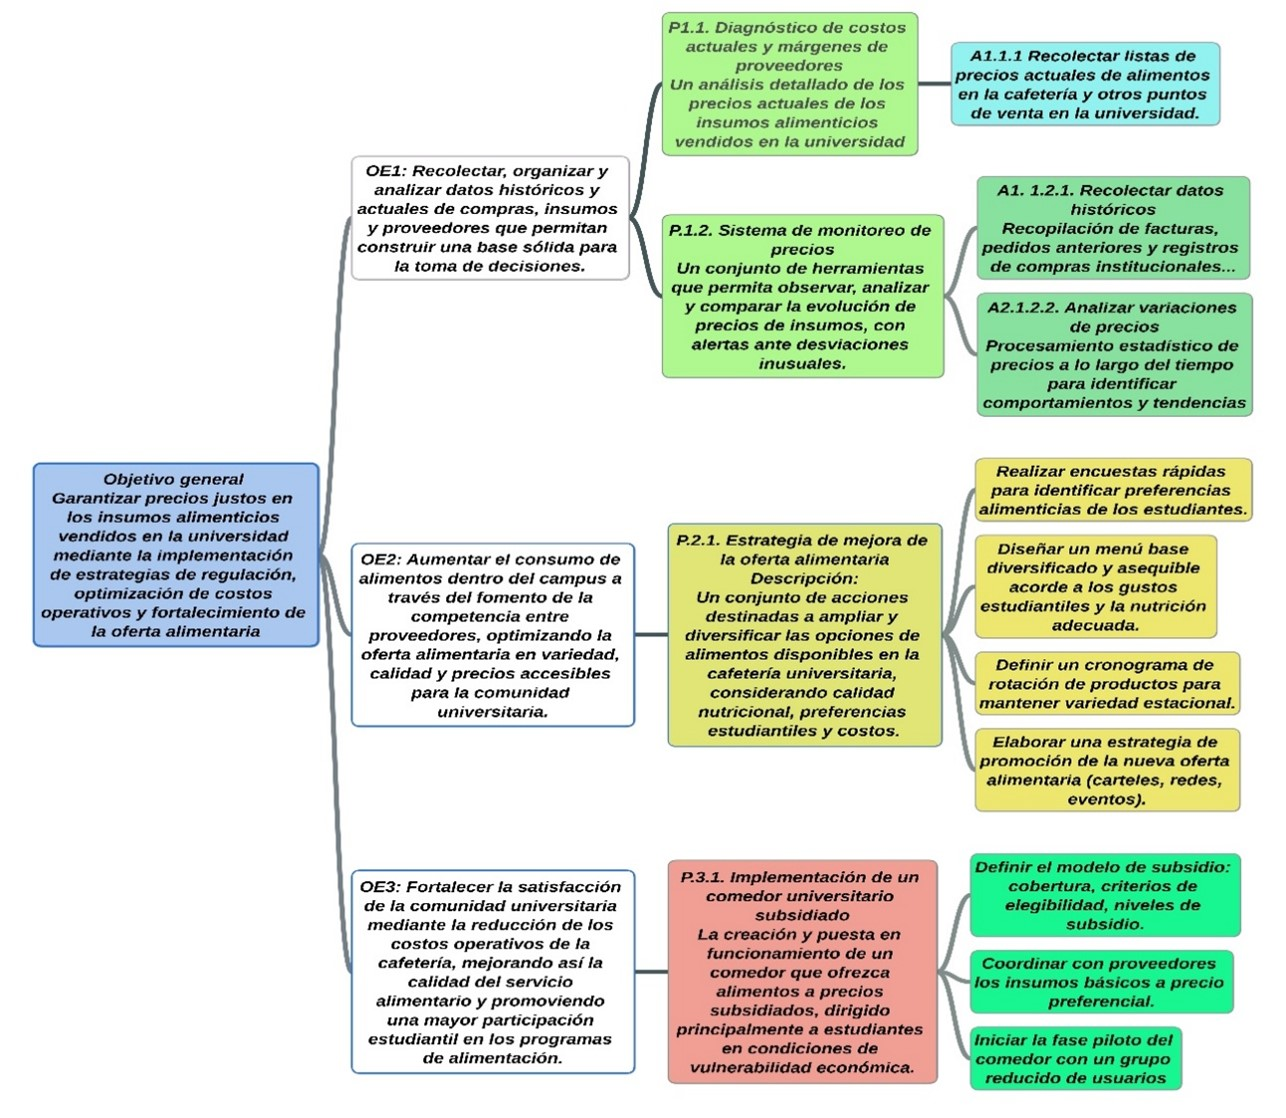
\includegraphics[width=.6\linewidth]{./Images/cadena_valor.jpg}
            \caption{}
      \end{center}
\end{figure}

\subsubsection{Cronograma de actividades}

\begin{figure}[H]
      \begin{center}
            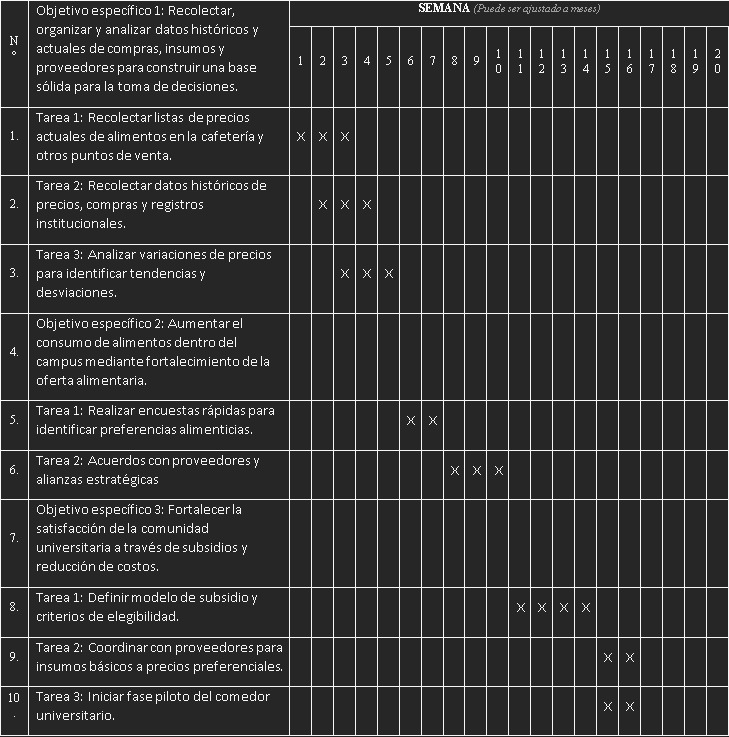
\includegraphics[width=\linewidth]{./Images/cronograma.jpg}
            \caption{}
      \end{center}
\end{figure}

\newpage
\subsubsection{Identificación y descripción de las tecnologías disponibles}

\begin{longtable}{|p{.3\linewidth}|p{.3\linewidth}|p{.3\linewidth}|}
      \caption{Matriz De Plan de Estudio}                                                                                                                                 \\
      \hline
      \textbf{Producto}                                                    & \textbf{Insumo}                                                        & \textbf{Tecnología} \\
      \hline
      \endfirsthead

      \hline
      \textbf{Producto}                                                    & \textbf{Insumo}                                                        & \textbf{Tecnología} \\
      \hline
      \endhead

      \hline
      \endfoot

      \hline
      \endlastfoot

      Estudio del uso de insumos y proveedores                             & Datos de compras, facturas
      anteriores, información de proveedores, inventario de alimentos      & Hojas de
      cálculo como Excel, sistemas de administración de compras.                                                                                                          \\\hline

      Creación de mecanismos de monitoreo y regulación de precios          & Listado de
      precios actuales, histórico de precios de insumos, datos de proveedores,
      encuestas estudiantiles.                                             & Herramientas de recolección de datos como Google
      Forms, hojas de cálculo en Excel con funciones de análisis                                                                                                          \\\hline

      Base de datos con proveedores y frecuencia de compra.                & Información recolectada
      sobre proveedores, fechas de pedidos, frecuencia de compras          & Bases de datos en
      Excel, SQL y formularios digitales con Google Forms.                                                                                                                \\\hline

      Creación de espacios competitivos para kioscos/concesionarios        & Precios de
      mercado, historial de compras, encuestas de satisfacción, informes anteriores.
                                                                           & Programas de informes como Power BI y procesadores de texto como Word.
      \\\hline

      Equipamiento del comedor (utensilios, mobiliario, electrodomésticos) & Estufas,
      hornos, licuadoras, mesas, sillas, neveras, utensilios (ollas, platos,
      cubiertos)                                                           & Equipos industriales o semiindustriales de cocina, tecnología de
      refrigeración, mobiliario de acero inoxidable.                                                                                                                      \\\hline

      Diseño de menús accesibles, balanceados nutricionalmente y adaptados a
      necesidades                                                          & Ingredientes locales, recetas nutricionales, requerimientos
      dietéticos (ej. vegetarianos, diabéticos)                            & Software de planificación
      nutricional como NutriSoft, hojas de cálculo con fórmulas calóricas.                                                                                                \\\hline
\end{longtable}

\subsection{Descripción del proceso productivo}

\subsubsection{Etapas}

\begin{enumerate}
      \item Estudio del Uso de Insumos y Proveedores \begin{itemize}
                  \item Objetivo: Analizar el consumo actual, identificar y clasificar proveedores
                        relevantes, evaluar la calidad y costos de insumos y detectar cuellos de
                        botella en la cadena de suministros.
            \end{itemize}

      \item Monitoreo y Regulación de Precios \begin{itemize}
                  \item Objetivo: Implementar un sistema tecnológico que permita la monitorización en
                        tiempo real de los precios de insumos y facilitar mecanismos para regularlos,
                        asegurando precios competitivos sin comprometer la calidad.
            \end{itemize}

      \item Análisis de Competitividad de Kioscos/Concesionarios \begin{itemize}
                  \item Objetivo: Evaluar la oferta y eficiencia de los concesionarios actuales y
                        comparar sus prácticas con las de potenciales nuevos actores del mercado.
            \end{itemize}

      \item Equipamiento del Comedor \begin{itemize}
                  \item Objetivo: Dotar al comedor de la tecnología y equipamiento necesarios para la
                        optimización operativa y el control de calidad.
            \end{itemize}

      \item Diseño de Menús Accesibles y Nutricionales \begin{itemize}
                  \item Objetivo: Desarrollar menús que respeten estándares nutricionales y sean
                        económicamente viables para la comunidad universitaria.
            \end{itemize}
\end{enumerate}

\newpage
\subsection{Asignación de Actividades}

\begin{longtable}{|c|p{.3\linewidth}|p{.3\linewidth}|p{.3\linewidth}|}
      \hline

      \textbf{Código}                                                           & \textbf{Actividad}                     & \textbf{Tecnología Apoyada} & \textbf{Dependencias} \\
      \hline
      \endfirsthead

      \hline

      \textbf{Código}                                                           & \textbf{Actividad}                     & \textbf{Tecnología Apoyada} & \textbf{Dependencias} \\
      \hline
      \endhead

      A                                                                         & Recolectar datos de compras y facturas & Excel, sistemas de compras  &
      Ninguna                                                                                                                                                                  \\ \hline B  & Analizar historial de precios y crear mecanismos de
      monitoreo                                                                 & Google Forms, Excel                    & A                                                   \\ \hline C                           & Crear base de datos de
      proveedores y frecuencia de compra                                        & Google Forms, SQL, Excel               & A                                                   \\ \hline D                                                        &
      Diseñar encuestas de satisfacción y levantar precios de mercado           & Google Forms,
      Power BI                                                                  & A                                                                                            \\ \hline E                             & Evaluar infraestructura del comedor (equipamiento) &
      Observación directa, fichas técnicas                                      & Ninguna                                                                                      \\ \hline F                 & Diseñar propuestas
      de equipamiento adecuado                                                  & Tecnología industrial                  & E                                                   \\ \hline G                         & Planear
      menús nutricionales y accesibles                                          & NutriSoft, Excel                       & B, C, D                                             \\ \hline H                                                                  &
      Redactar informe final con propuestas de regulación y nutrición accesible &
      Word, Power BI                                                            & F, G                                                                                         \\ \hline

      \caption{Actividades, tecnologías utilizadas y dependencias}
\end{longtable}

\newpage
\subsection{Duraciones Estimadas por Actividad}

\begin{longtable}{|c|p{.6\linewidth}|c|}
      \hline

      \textbf{Código}                               & \textbf{Actividad}                     & \textbf{Duración (días)} \\
      \hline
      \endfirsthead

      \hline

      \textbf{Código}                               & \textbf{Actividad}                     & \textbf{Duración (días)} \\
      \hline
      \endhead

      A                                             & Recolectar datos de compras y facturas & 3                        \\ \hline B                                   & Analizar historial
      de precios y crear mecanismos de monitoreo    & 2                                                                 \\ \hline C                                    & Crear base de
      datos de proveedores y frecuencia de compra   & 3                                                                 \\ \hline D                                      & Diseñar encuestas
      de satisfacción y levantar precios de mercado & 2                                                                 \\ \hline E                                   & Evaluar
      infraestructura del comedor (equipamiento)    & 1                                                                 \\ \hline F                 & Diseñar propuestas
      de equipamiento adecuado                      & 2                                                                 \\ \hline G   & Planear menús nutricionales y
      accesibles                                    & 4                                                                 \\ \hline H                         & Redactar informe final con propuestas de
      regulación y nutrición accesible              & 3                                                                 \\ \hline

      \caption{Duración estimada de cada actividad}
\end{longtable}

A continuación, teniendo en cuenta los pasos anteriores, realizamos las
relaciones de precedencia.

\subsection{Relaciones de Precedencia}

\begin{itemize}[label=$\triangleright$]
      \item  $A \rightarrow B, C, D$
      \item  $B, C, D \rightarrow G$
      \item  $E \rightarrow F$
      \item  $F, G \rightarrow H$

\end{itemize}

\subsection{Cálculo de la Ruta Crítica}

Procedemos a identificar todos los caminos posibles y calcular sus duraciones
totales:

\begin{itemize}
      \item Camino 1: $A \rightarrow B \rightarrow G \rightarrow H$ \\ A (3) + B (2) + G
            (4) + H (3) = 12 días.

      \item Camino 2: $A \rightarrow C \rightarrow G \rightarrow H$ \\ A (3) + C (3) + G
            (4) + H (3) = 13 días.

      \item Camino 3: $A \rightarrow D \rightarrow G \rightarrow H$ \\ A (3) + D (2) + G
            (4) + H (3) = 12 días.

      \item Camino 4: $E \rightarrow F \rightarrow H$ \\ E (1) + F (2) + H (3) = 6 días.
\end{itemize}

Luego de realizar los cálculos, la ruta crítica seleccionada es el camino 2, el
cual es el más largo, elegimos este porque es la única secuencia de actividades
cuya duración completa (13 días) define directamente la duración total del
proyecto. Si alguna de estas tareas se retrasa, el proyecto entero se retrasa.
Con esto nos queda que las actividades en la ruta crítica son las siguientes:

\begin{itemize}
      \item A (Recolectar datos de compras).
      \item C (Crear base de datos de proveedores).
      \item G (Planear menús nutricionales).
      \item H (Redactar informe final).
\end{itemize}

\subsection{Esquemático del Diagrama del Método de la ruta crítica (CPM)}

\begin{figure}[H]
      \begin{center}
            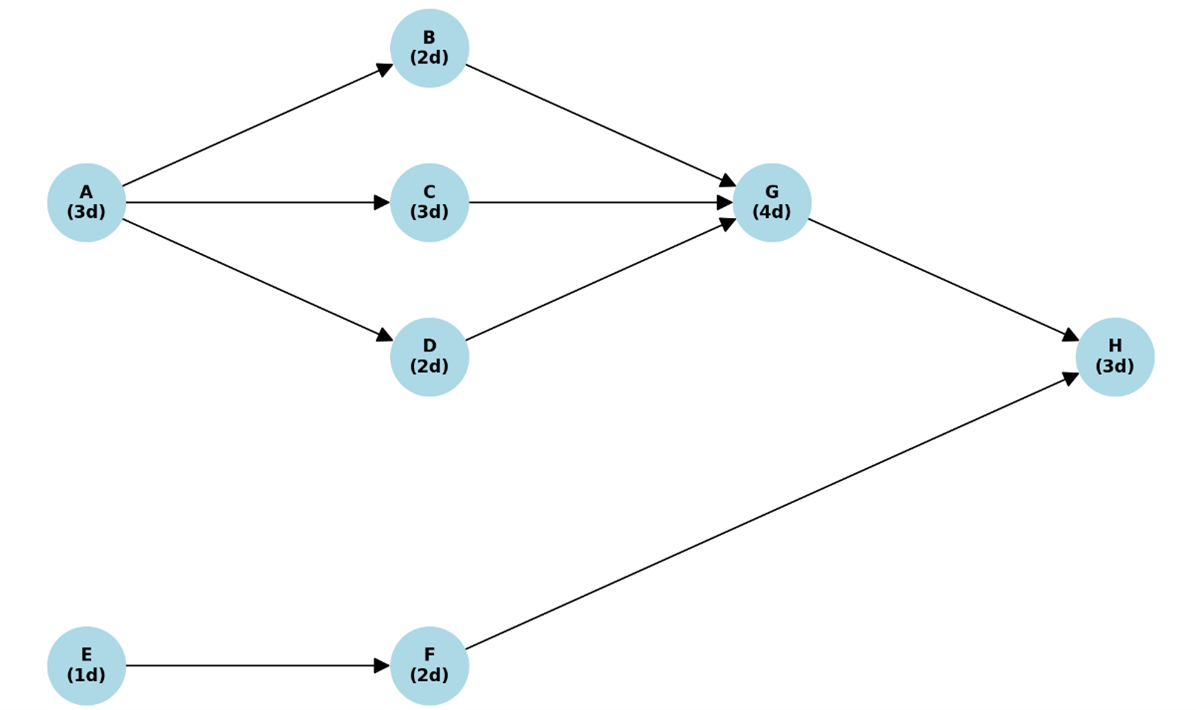
\includegraphics[width=\linewidth]{./Images/diagrama_idk.png}
            \caption{}
      \end{center}
\end{figure}

\subsubsection{Especificaciones técnicas y de modelo}

\begin{longtable}{|p{.5\linewidth}|p{.5\linewidth}|}
      \hline

      \textbf{Área}                          & \textbf{Especificaciones Técnicas}                        \\
      \hline
      \endfirsthead

      \hline

      \textbf{Área}                          & \textbf{Especificaciones Técnicas}                        \\
      \hline
      \endhead

      Base de datos de insumos y proveedores & Capacidad para almacenar más de 500
      registros. Acceso restringido a usuarios autorizados. Actualización semestral
      de la información. Compatibilidad con Excel y SQL.                                                 \\\hline

      Sistema de monitoreo de precios        & Visualización de precios actualizados
      semanalmente.- Generación automática de alertas al superar variaciones del 10\%
      en precios. Interfaz gráfica amigable compatible con Power BI. Respaldo
      automático de los datos cada 15 días.                                                              \\\hline

      Equipamiento del comedor               & Equipos de cocina industrial de acero inoxidable.
      Refrigeradores energéticamente eficientes (certificación Energy Star).
      Cumplimiento de normativas de inocuidad alimentaria (ISO 22000).- Mobiliario de
      fácil limpieza y alta durabilidad.                                                                 \\\hline

      Menús accesibles y nutricionales       & Desarrollo de menús adaptados a necesidades
      especiales (vegetarianos, diabéticos). Cálculo de valor nutricional en cada
      menú (uso de NutriSoft). Inclusión de opciones con precios accesibles para
      estudiantes.                                                                                       \\\hline

      Proveedores                            & Evaluación anual de calidad y cumplimiento.- Contratos de
      suministro con cláusulas de precios regulados. Capacidad de abastecimiento
      continuo en condiciones de alta demanda.                                                           \\\hline
\end{longtable}

\subsection{Modelo}

Se propone un modelo de flujo de proceso que represente el funcionamiento del
sistema de regulación de precios de insumos alimentarios:

\begin{enumerate}
      \item Ingreso de datos \begin{itemize}
                  \item Recolección de precios de insumos mediante formularios digitales.
            \end{itemize}

      \item Actualización de base de datos \begin{itemize}
                  \item Consolidación automática en una plataforma de base de datos (Excel/SQL).
            \end{itemize}

      \item Análisis de precios \begin{itemize}
                  \item Comparación de precios actuales vs históricos.
                  \item Detección de variaciones significativas.

            \end{itemize}

      \item Alertas y reportes \begin{itemize}
                  \item Emisión de alertas a administradores si se detectan incrementos atípicos.
                  \item Generación de reportes mensuales de precios y proveedores.

            \end{itemize}

      \item Decisiones y ajustes \begin{itemize}
                  \item Toma de decisiones para ajustes de proveedores, negociaciones o intervenciones.
            \end{itemize}

      \item Monitoreo continuo \begin{itemize}
                  \item Seguimiento permanente de precios, calidad de insumos y satisfacción
                        estudiantil.
            \end{itemize}
\end{enumerate}

Este modelo puede representarse gráficamente mediante un diagrama de bloques de
flujo, enlazando cada uno de estos pasos.

\begin{figure}[H]
      \begin{center}
            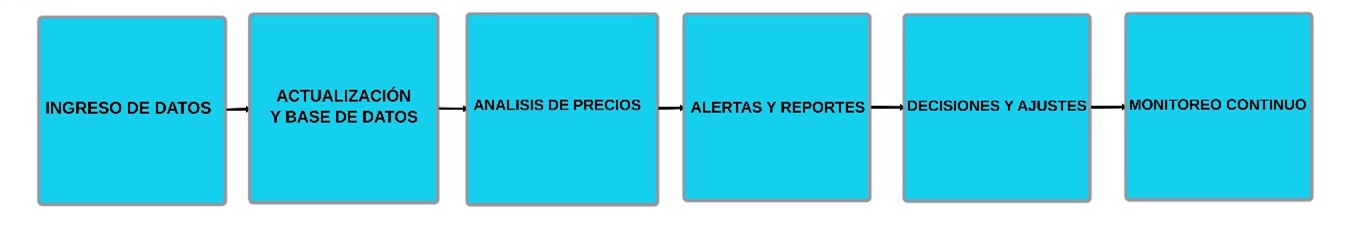
\includegraphics[width=\linewidth]{./Images/diagrama_bloques.jpg}
            \caption{Diagrama de Bloques - Modelo del Sistema de Regulación de Precios Alimentarios}
      \end{center}
\end{figure}

\section{Planificación Financiera}

\subsection{Cronograma de Actividades (20 meses)}

\noindent\textbf{Presupuesto asignado: \$120.000.000 COP}

\vspace{0.5cm}

\begin{longtable}{|c|p{.4\linewidth}|p{.2\linewidth}|p{.2\linewidth}|}
      \hline

      \textbf{Fase}  & \textbf{Actividades Clave}                      & \textbf{Duración (Meses)} & \textbf{Responsable}    \\
      \hline
      \endfirsthead

      \hline

      \textbf{Fase}  & \textbf{Actividades Clave}                      & \textbf{Duración (Meses)} & \textbf{Responsable}    \\
      \hline
      \endhead

      1. Diagnóstico & Encuestas digitales, estudio de precios         & 0 -- 3                    & Equipo de investigación \\
      \hline
      2. Políticas   & Negociación con proveedores, diseño del comedor & 4 -- 6                    & Administración          \\
      \hline
      3. Ejecución   & Regulación de precios, apertura del comedor     & 7 -- 12                   & Operaciones             \\
      \hline
      4. Monitoreo   & Evaluaciones trimestrales, ajustes operativos   & 13 -- 20                  & Auditoría               \\
      \hline

      \caption{Fases del proyecto con duración y responsables}
\end{longtable}

\subsection{Presupuesto Detallado (COP)}

\subsubsection{Tecnología}

\begin{longtable}{|p{.25\linewidth}|p{.25\linewidth}|p{.25\linewidth}|p{.25\linewidth}|}
      \hline
      \textbf{Ítem}             & \textbf{Descripción}                      & \textbf{Costo Unitario} & \textbf{Subtotal}    \\
      \hline
      Software de monitoreo     & Licencia anual (Ej: SIESCO)               & \$3.500.000             & \$3.500.000          \\
      \hline
      Eliminación de app móvil  & Se utilizarán encuestas en redes sociales & -                       & \$0                  \\
      \hline
      \textbf{Total Tecnología} &                                           &                         & \textbf{\$3.500.000} \\
      \hline
\end{longtable}

\subsubsection{Costos Operativos}

\begin{longtable}{|p{0.25\linewidth}|p{0.35\linewidth}|p{0.20\linewidth}|p{0.20\linewidth}|}
      \hline
      \textbf{Etapa}            & \textbf{Descripción}                               & \textbf{Costo Unitario} & \textbf{Subtotal}    \\
      \hline
      Encuestas en redes        & Realizadas por estudiantes                         & \$0                     & \$0                  \\
      \hline
      Talleres a proveedores    & Capacitación en estándares alimentarios (2 al año) & \$1.200.000             & \$2.400.000          \\
      \hline
      \textbf{Total Operativos} &                                                    &                         & \textbf{\$2.400.000} \\
      \hline
\end{longtable}

\subsubsection{Comedor Subsidiado}

\begin{longtable}{|p{0.25\linewidth}|p{0.35\linewidth}|p{0.20\linewidth}|p{0.20\linewidth}|}
      \hline
      \textbf{Ítem}             & \textbf{Descripción}                       & \textbf{Costo Unitario} & \textbf{Subtotal}     \\
      \hline
      Mobiliario y equipamiento & Mesas, sillas, cocina industrial           & \$15.000.000            & \$15.000.000          \\
      \hline
      Subsidios alimentarios    & 200 estudiantes por 6 meses (\$50.000/mes) &                         & \$60.000.000          \\
      \hline
      \textbf{Total Comedor}    &                                            &                         & \textbf{\$75.000.000} \\
      \hline
\end{longtable}

\subsubsection{Resumen General}
\begin{longtable}{|p{0.6\linewidth}|p{0.4\linewidth}|}
      \hline
      \textbf{Categoría}      & \textbf{Monto (COP)}  \\
      \hline
      Total parcial           & \$80.900.000          \\
      \hline
      10\% imprevistos        & \$12.000.000          \\
      \hline
      \textbf{Total estimado} & \textbf{\$92.900.000} \\
      \hline
\end{longtable}

Nota: El 10\% de los imprevistos incluyen los factores externos los cuales
pueden afectar al costo principal del proyecto.

\subsection{Proveedores Locales}

\subsubsection{Tecnología}

\begin{longtable}{|p{0.2\linewidth}|p{0.3\linewidth}|p{0.3\linewidth}|p{0.2\linewidth}|}
      \hline
      \textbf{Empresa} & \textbf{Servicio}  & \textbf{Contacto}      & \textbf{Ventaja Competitiva} \\
      \hline
      SIESCO           & Software educativo & contacto@siesco.com.co &
      Especialización en educación                                                                  \\\hline

\end{longtable}

\subsubsection{Alimentos y Logística - Análisis de Ventajas Competitivas}

\begin{longtable}{|p{0.15\linewidth}|p{0.20\linewidth}|p{0.25\linewidth}|p{0.15\linewidth}|p{0.20\linewidth}|}
      \hline
      \textbf{Proveedor}                                                                                                      & \textbf{Producto o Servicio} & \textbf{Contacto}                                                                                      & \textbf{Ventaja Competitiva} & \textbf{Comparación con Alternativas} \\
      \hline
      Alimentos Turbo                                                                                                         & Distribución de insumos      & Tel: 300 555 1234 \hfil \break Correo: ventas@alimentosturbo.co                                        &
      Precios 15--20\% más bajos que mayoristas nacionales. \hfil \break Entrega en 24h en Turbaco.                           &
      Distribuidora Súper: Precios altos por intermediarios. \hfil \break Éxito/Makro: Logística lenta (3--5 días).                                                                                                                                                                                                                          \\
      \hline
      Café Colombia                                                                                                           & Café y snacks orgánicos      & Tel: 318 555 5678 \hfil \break Correo: pedidos@cafecolombia.co                                         &
      Certificación Rainforest Alliance. \hfil \break Empaques biodegradables y devoluciones.                                 &
      Juan Valdez: Más costoso, sin empaques ecológicos. \hfil \break Café Quindío: Sin cobertura en Bolívar.                                                                                                                                                                                                                                \\
      \hline
      Frutas del Caribe                                                                                                       & Frutas/verduras frescas      & Tel: 320 555 9012 \hfil \break Correo: info@frutasdelcaribe.co                                         &
      Directo de fincas locales (huella de carbono reducida). \hfil \break 10\% descuento por volumen (\textgreater\$5M COP). &
      Corabastos: Precios variables + alto costo de transporte desde Bogotá.                                                                                                                                                                                                                                                                 \\
      \hline
      Panadería La Especial                                                                                                   & Pan artesanal                & Tel: 315 555 3456 \hfil \break Correo: \hfil{} \break{} pedidos\hfil{} \break{}@panaderialaespecial.co &
      Precios 30\% menores que pan industrial. \hfil \break Opciones sin gluten/integral.                                     &
      Bimbo\hfil{} \break{} /Supermercados: Pan precocido, menos fresco y sin personalización.                                                                                                                                                                                                                                               \\
      \hline
\end{longtable}

\subsection{Análisis Detallado de Ventajas}

\begin{enumerate}
      \item Costos Logísticos \begin{itemize}
                  \item Proveedores locales: \begin{itemize}
                              \item Ahorro del 25% en transporte (ej: Alimentos Turbo opera en Turbaco; no requiere fletes desde Barranquilla/Bogotá).
                              \item Menos pérdidas por caducidad (distancias cortas = alimentos más frescos).

                        \end{itemize}

                  \item Alternativas externas: \begin{itemize}
                              \item Costos adicionales por combustible y peajes (ej: envíos desde Medellin).
                        \end{itemize}
            \end{itemize}

      \item Calidad y Sostenibilidad \begin{itemize}
                  \item Café Colombia: \begin{itemize}
                              \item Certificación Rainforest Alliance (no ofrecida por competidores regionales).
                              \item Empaques biodegradables (competencia usa plástico).
                        \end{itemize}

                  \item Frutas del Caribe: \begin{itemize}
                              \item "Del campo a la universidad": Menos intermediarios = mejor precio y apoyo a agricultores locales.
                        \end{itemize}
            \end{itemize}

      \item Flexibilidad y Servicio \begin{itemize}
                  \item Pedidos personalizados: \begin{itemize}
                              \item Panadería La Especial ajusta recetas para estudiantes con dietas especiales
                                    (veganos, celíacos).
                        \end{itemize}

                  \item  Respuesta rápida: \begin{enumerate}
                              \item Priorizar convenios con proveedores locales para garantizar sostenibilidad.
                              \item Formalizar contrato con SIESCO antes del mes 4.
                              \item Implementar control de gastos mensual con herramientas contables como Siigo.
                        \end{enumerate}
            \end{itemize}
\end{enumerate}

\section{Macro localización y Micro localización del Proyecto}

\subsection{Macro localización}

Zona: Campus principal de la UTB en la sede Turbaco.

Factores clave: \begin{itemize}
      \item Alta demanda de estudiantes.
      \item Infraestructura existente (cafeterías, áreas comunes).

\end{itemize}

\subsection{Micro localización}

\begin{longtable}{|p{0.25\linewidth}|p{0.35\linewidth}|p{0.35\linewidth}|}
      \hline
      \textbf{Espacio}     & \textbf{Uso en el Proyecto}       & \textbf{Ventajas}             \\
      \hline
      \endfirsthead

      \hline
      \textbf{Espacio}     & \textbf{Uso en el Proyecto}       & \textbf{Ventajas}             \\
      \hline
      \endhead

      Comedor central      & Comedor subsidiado                & Capacidad para 200+ personas. \\ \hline
      Oficina de bienestar & Gestión de políticas y auditorías & Proximidad a la
      administración.                                                                          \\ \hline Cafetería 1 (entrada) & Pilotaje de regulación de
      precios              & Mayor flujo de estudiantes.                                       \\ \hline

\end{longtable}

\section{Metodología utilizada}

Durante un semestre universitario, que normalmente dura unas 16 semanas, los
estudiantes deben asumir diferentes tipos de gastos, como transporte,
alimentación, recreación, entre otros. Teniendo esto en cuenta, es común que a
mitad de semestre muchos se enfrenten a dificultades económicas que los obligan
a buscar alternativas. Por ejemplo, puede que ya no les alcance para el
transporte diario y deban buscar otras opciones, o que no puedan seguir pagando
los almuerzos en la universidad y tengan que empezar a cocinar en casa cada
mañana.

El objetivo de este trabajo es representar gráficamente cómo varía el balance
económico de un estudiante a lo largo del semestre. Para lograrlo, se
realizaron simulaciones utilizando parámetros definidos desde un software, con
el fin de visualizar estos cambios de manera más clara,
planteando lo siguiente:

\begin{figure}[H]
      \begin{center}
            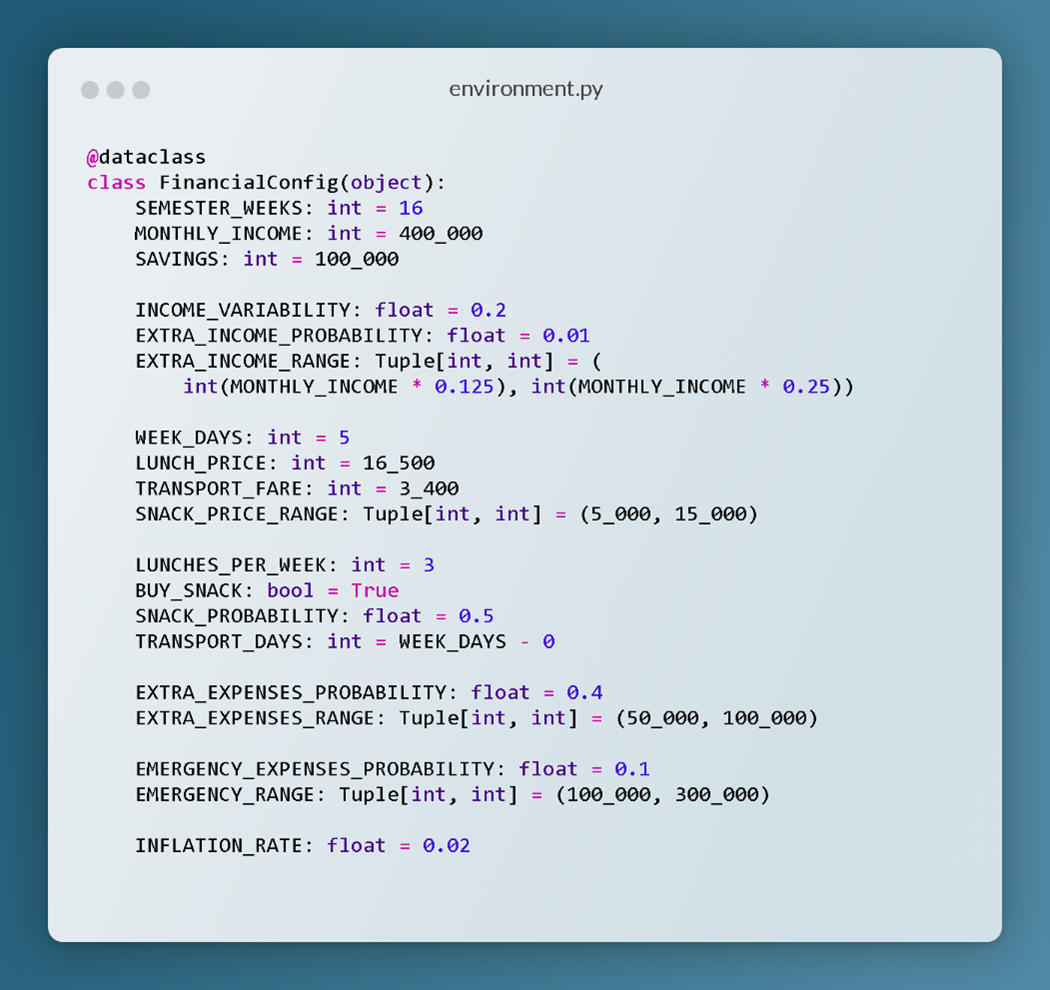
\includegraphics[width=\linewidth]{./Images/environment_snippet.png}
            \caption{}
      \end{center}
\end{figure}

El snippet de arriba nos permite visualizar todos los parámetros de la
simulación. A continuación, se describen los aspectos más relevantes:

\begin{itemize}
      \item \texttt{SEMESTER\_WEEKS}, cantidad de semanas en un semestre
      \item \texttt{MONTHLY\_INCOME}, ganancias mensuales del estudiante, asimismo, \texttt{SAVINGS}, declara los ahorros iniciales del mismo.
      \item \texttt{EXTRA\_INCOME\_RANGE}, establece el rango para gastos “extra” que se puedan presentar en el semestre. \texttt{EMERGENCY\_RANGE}, cumple con la misma función, apuntando a gastos de “emergencia”.
      \item Luego ciertas variables del entorno como por ejemplo \texttt{LUNCH\_PRICE}
            (valor del almuerzo), \texttt{SNACK\_PRICE\_RANGE} (rango de precios de una
            merienda), \texttt{TRANSPORT\_FARE} (valor del transporte).
\end{itemize}

Un punto importante para mencionar es que, no se puede esperar que la
simulación retorne siempre el mismo output, de tal manera que se construye en
base a probabilidades, una de ellas siendo \texttt{INFLATION\_RATE}.

\begin{figure}[H]
      \begin{center}
            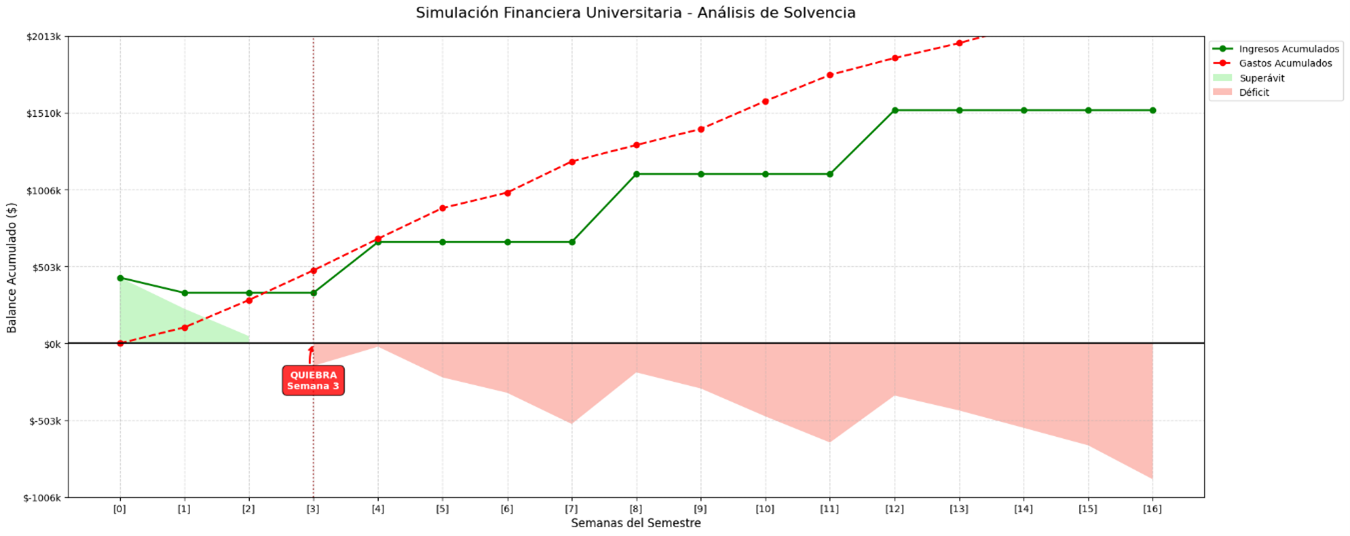
\includegraphics[width=\linewidth]{./Images/output_sample.png}
            \caption{}
      \end{center}
\end{figure}

Como podemos notar, se presenta un ejemplo de simulación, el cual esta
compuesto por varias parte, que son las siguientes:

\begin{itemize}
      \item Sombreado Verde y Rojo: Encargados de mostrar como se comporta en balance
            actual del estudiante
      \item Línea Roja: Representa los gastos del semestre. Como se puede observar, no
            siempre es una ``línea recta''.
      \item Línea Verde: Representa los ingresos del estudiante a lo largo del semestre.
\end{itemize}

Los datos usados para generar la simulación son meramente ficticios, con la
excepción de algunos parámetros relacionados al entorno. De igual manera, la
herramienta nos permite identificar patrones que serán útiles a futuro.

% \section{Conclusión}

% La reducción de los precios de los insumos alimenticios en la universidad es un
% problema de alto impacto para la comunidad estudiantil. Mediante estrategias
% como la regulación de precios, el fomento de la competencia y la creación de un
% comedor subsidiado es posible mejorar el acceso a una alimentación de calidad y
% reducir la carga económica sobre los estudiantes. La implementación de estas
% medidas requiere un esfuerzo coordinado entre la administración universitaria,
% proveedores y organismos de control, pero traerá beneficios significativos en
% la calidad de vida y el rendimiento académico de los estudiantes.

% \newpage
% \printbibliography

\section{Estudios}

\subsection{Estudio Ambiental}

\subsubsection{Tipo de Impacto Ambiental}

El proyecto se clasifica como de bajo impacto ambiental, ya que: 

\begin{itemize}
      \item No involucra actividades extractivas, construcción de infraestructura 
      pesada o alteración de ecosistemas. 
      
      \item Sus impactos son controlables mediante buenas prácticas ambientales. 
\end{itemize}

\subsubsection{Instrumentos para Identificar y Estudiar el Impacto Ambiental}

\paragraph{Estudio de Linea Base}
\begin{itemize}
      \item \textbf{Diagnóstico inicial}: Evaluación del estado actual del campus en 
      términos de: 
            \begin{itemize}
                  \item Consumo de energía y agua en cafeterías existentes. 
                  \item Generación de residuos sólidos (orgánicos y empaques). 
                  \item Huella de carbono por transporte de insumos. 
            \end{itemize}
\end{itemize}

\paragraph{Matriz de Leopold (Ejemplo)}

\begin{itemize}
      \item Actividades principales del proyecto: \begin{itemize}
            \item Variables ambientales afectadas. 
            \item Magnitud (impacto físico/tangible) de 1 a 10. 
            \item Importancia (relevancia para el entorno) de 1 a 10. 
            \item Tipo de impacto (positivo o negativo). 
            \item Comentarios técnicos sobre el posible efecto ambiental. 
      \end{itemize}
\end{itemize}

\begin{longtable}{|>{\raggedright\arraybackslash}p{0.18\linewidth}|>{\raggedright\arraybackslash}p{0.18\linewidth}|>{\centering\arraybackslash}p{0.06\linewidth}|>{\centering\arraybackslash}p{0.08\linewidth}|>{\centering\arraybackslash}p{0.12\linewidth}|>{\raggedright\arraybackslash}p{0.24\linewidth}|}
\caption{Evaluación de Impactos Ambientales del Proyecto de Comedor} \\
\hline
\textbf{Actividad del Proyecto} & \textbf{Variable Ambiental Afectada} & \textbf{I\footnotemark[1]} & \textbf{II\footnotemark[2]} & \textbf{Tipo de Impacto} & \textbf{Comentarios} \\
\hline
\endfirsthead

\hline
\textbf{Actividad del Proyecto} & \textbf{Variable Ambiental Afectada} & \textbf{I\footnotemark[1]} & \textbf{II\footnotemark[2]} & \textbf{Tipo de Impacto} & \textbf{Comentarios} \\
\hline
\endhead

Operación del comedor (preparación, servicio) & 
Generación de residuos orgánicos & 
6 & 
7 & 
Negativo & 
Puede generar problemas de disposición si no se implementa compostaje o separación en la fuente. \\
\hline

Uso de equipos de cocina eléctricos & 
Consumo de energía & 
5 & 
6 & 
Negativo & 
Aumenta el consumo eléctrico, pero puede mitigarse con uso de equipos eficientes. \\
\hline

Refrigeración de alimentos & 
Emisiones indirectas (uso de energía) & 
4 & 
6 & 
Negativo & 
Emisiones por consumo de electricidad de refrigeradores si no se usan tecnologías eficientes. \\
\hline

Transporte de insumos & 
Emisión de gases contaminantes & 
3 & 
5 & 
Negativo & 
Con proveedores locales, se puede reducir este impacto. \\
\hline

Uso de agua en lavado y cocina & 
Consumo de recurso hídrico & 
5 & 
7 & 
Negativo & 
Se requiere implementación de dispositivos de bajo consumo. \\
\hline

Disposición de empaques & 
Generación de residuos inorgánicos & 
6 & 
6 & 
Negativo & 
Si se utilizan empaques biodegradables o reutilizables, el impacto se reduce. \\
\hline

Implementación de compostaje & 
Calidad del suelo & 
4 & 
5 & 
Positivo & 
Mejora el manejo de residuos orgánicos y enriquece el suelo si se aplica localmente. \\
\hline

Instalación de paneles solares & 
Reducción de consumo de energía convencional & 
5 & 
6 & 
Positivo & 
Contribuye al uso de energías limpias y reduce la huella de carbono del comedor. \\
\hline

Gestión adecuada de los aceites de cocina usados (ACU) & 
Recurso hídrico & 
6 & 
7 & 
Positivo & 
Promoción del desarrollo sostenible implementado buenas prácticas ambientales \\
\hline

Educación ambiental a la comunidad & 
Conciencia ambiental & 
2 & 
8 & 
Positivo & 
Impacto directo en la cultura ambiental universitaria a largo plazo. \\
\hline

Restauración del espacio (en caso de cierre) & 
Uso de suelo y paisaje & 
3 & 
4 & 
Negativo & 
El área debe restaurarse al estado inicial si el proyecto se desmonta. \\
\hline

\end{longtable}
\footnotetext[1]{Magnitud (1-10)}
\footnotetext[2]{Importancia (1-10)}

\paragraph{Notas para el analisis}
\begin{itemize}
      \item Impactos negativos predominan durante la operación, pero pueden ser mitigados con estrategias ambientales adecuadas como compostaje, separación de residuos y energías limpias. 

      \item La inclusión de acciones educativas y sostenibles da lugar a impactos positivos que fortalecen el desempeño ambiental del proyecto. 

      \item Se recomienda realizar monitoreo periódico para evaluar si las medidas de mitigación están siendo efectivas. 
\end{itemize}

\subsubsection{Demanda Ambiental}

\paragraph{Recursos Utilizados}
\begin{itemize}
      \item Agua: Lavado de utensilios y preparación de alimentos. 
      \item Energía: Refrigeración, iluminación y equipos de cocina. 
      \item Materiales: Empaques (plástico, cartón) y utensilios desechables. 
\end{itemize}

\paragraph{Flujos de residuos}
\begin{itemize}
      \item Residuos Solidos:
            \begin{itemize}
                  \item Orgánicos (restos de comida). 
                  \item Inorgánicos (empaques, plásticos). 
            \end{itemize}
      \item Gestión adecuada de los Acu (Aceite de cocina usados) 
\end{itemize}

\paragraph{Consumo Energetico}
\begin{itemize}
      \item Iluminación LED en puntos de venta. 
      \item Equipos de cocina eficientes (certificación Energy Star). 
\end{itemize}

\paragraph{Uso de Espacio Fisico}
\begin{itemize}
      \item Ocupación de áreas comunes del campus (ej.:\@{}comedor central). 
\end{itemize}

\subsubsection{Marco Legal-Ambiental}

\paragraph{Permisos Requeridos}
\begin{itemize}
      \item Permiso de vertimientos: Si las aguas residuales generadas se vierten a cuerpos de agua.
      \item Certificación de higiene alimentaria.
\end{itemize}

\paragraph{Gestión}
\begin{itemize}
      \item Gestión integral de los residuos sólidos generados.
      \item Gestión de los aceites de cocina usados.
\end{itemize}

\paragraph{Programas}
\begin{itemize}
      \item Programa de uso eficiente de energía.
      \item Programa de ahorro de agua.
\end{itemize}

\paragraph{Normativas Aplicables}
\begin{itemize}
      \item Ley 99 de 1993 (Crea el Ministerio del Ambiente y el Sistema Nacional Ambiental).
      \item Resolución 0631 de 2015 (Establece los parámetros para vertimiento).
      \item Resolución 316 de 2018 (Establece disposiciones para la gestión de los aceites de cocina usados).
      \item Ley 2232 (Define la eliminación de 21 plásticos de un solo uso para el 2030).
      \item Resolución 2184 del 2019 (Establece el código de colores para la separación de los residuos en la fuente).
\end{itemize}

\subsubsection{Costos Ambientales}

\paragraph{Durante la Operación}
\begin{itemize}
      \item Consumo energético: \$2.400.000 COP anuales (iluminación y refrigeración).
      \item Gestión de residuos: \$1.500.000 COP anuales (reciclaje y disposición).
      \item Transporte sostenible: Incentivos para proveedores locales (\$500.000 COP).
\end{itemize}

\paragraph{Cierre o Desmantelamiento}
\begin{itemize}
      \item Retiro de mobiliario y equipos (\$3.000.000 COP).
      \item Restauración de áreas comunes (\$1.000.000 COP).
\end{itemize}

\subsubsection{Medidas de Mitigación y Plan de Manejo Ambiental}

\paragraph{Prevención}
\begin{itemize}
      \item Energía: Instalación de paneles solares para el comedor.
      \item Agua: Uso de sistemas de bajo consumo (grifos automáticos).
\end{itemize}

\paragraph{Mitigación}
\begin{itemize}
      \item Residuos:
            \begin{itemize}
                  \item Programa de separación en la fuente (orgánicos/inorgánicos).
                  \item Compostaje de residuos orgánicos.
            \end{itemize}
      \item Emisiones: Priorizar proveedores locales para reducir transporte.
\end{itemize}

\paragraph{Monitoreo}
\begin{itemize}
      \item Auditorías semestrales de consumo energético y generación de residuos.
      \item Encuestas de satisfacción ambiental a la comunidad universitaria.
\end{itemize}

\subsubsection{Criterios de Evaluación}

\paragraph{Protección de Ecosistemas}
\begin{itemize}
      \item No afecta áreas naturales protegidas.
\end{itemize}

\paragraph{Uso Eficiente de Recursos}
\begin{itemize}
      \item Promueve energía renovable y reducción de residuos.
\end{itemize}

\paragraph{Gestión de Residuos}
\begin{itemize}
      \item Cumple con normativas locales.
\end{itemize}

\paragraph{Participación Comunitaria}
\begin{itemize}
      \item Incluye campañas de concientización ambiental.
\end{itemize}

\end{document}